%\documentclass[handout]{beamer} %Il faut enlever [handout] pour avoir les transitions
\documentclass{beamer} %Il faut enlever [handout] pour avoir les transitions
\usepackage[utf8]{inputenc}
\usepackage[frenchb]{babel}
\usetheme{Warsaw}
\title{Développement d'interface graphique avec Qt}
\author{
Vincent Barichard \\ %repris par Jean-Mathieu Chantrein
}

\usepackage{lmodern}

\institute{LERIA - Université d'Angers}
\date{ %13 juin 2014 \\ \vspace{1.5cm}\large{JIAF 2014}}
\today}
\setbeamercovered{invisible}

\setbeamertemplate{navigation symbols}{}
\addtobeamertemplate{footline}{\hfill\insertframenumber/\inserttotalframenumber\hspace{2em}\null}

\usepackage{array,multirow,rotating,hhline,subfig}
\usepackage{amsmath,amssymb,mathrsfs}
\usepackage{float}
\usepackage{graphicx}
\usepackage{tikz}
\usetikzlibrary{fit,decorations.pathmorphing,arrows,shapes}

% Debut Ecriture et la coloration syntaxique de code
\usepackage{listings} 
\lstdefinestyle{customcpp}{
  %belowcaptionskip=0\baselineskip,
  %escapeinside={(?}{?)},
  basicstyle=\scriptsize\ttfamily,
  %extendedchars=true,
  %breaklines=true,
  %frame=L,
  %xleftmargin=\parindent,
  language=C++,
  showstringspaces=false,
  %basicstyle=\footnotesize\ttfamily,
  keywordstyle=\bfseries\color{green!40!black},
  commentstyle=\color{purple!40!black},
  identifierstyle=\color{blue},
  stringstyle=\color{orange},
  tabsize=4,
  otherkeywords={signals,SIGNAL,slots,SLOT,Q_OBJECT}
}

\lstset{escapechar=@,style=customcpp}

\lstset{literate=
{á}{{\'a}}1 {é}{{\'e}}1 {í}{{\'i}}1 {ó}{{\'o}}1 {ú}{{\'u}}1
{Á}{{\'A}}1 {É}{{\'E}}1 {Í}{{\'I}}1 {Ó}{{\'O}}1 {Ú}{{\'U}}1
{à}{{\`a}}1 {è}{{\`e}}1 {ì}{{\`i}}1 {ò}{{\`o}}1 {ù}{{\`u}}1
{À}{{\`A}}1 {È}{{\'E}}1 {Ì}{{\`I}}1 {Ò}{{\`O}}1 {Ù}{{\`U}}1
{ä}{{\"a}}1 {ë}{{\"e}}1 {ï}{{\"i}}1 {ö}{{\"o}}1 {ü}{{\"u}}1
{Ä}{{\"A}}1 {Ë}{{\"E}}1 {Ï}{{\"I}}1 {Ö}{{\"O}}1 {Ü}{{\"U}}1
{â}{{\^a}}1 {ê}{{\^e}}1 {î}{{\^i}}1 {ô}{{\^o}}1 {û}{{\^u}}1
{Â}{{\^A}}1 {Ê}{{\^E}}1 {Î}{{\^I}}1 {Ô}{{\^O}}1 {Û}{{\^U}}1
{œ}{{\oe}}1 {Œ}{{\OE}}1 {æ}{{\ae}}1 {Æ}{{\AE}}1 {ß}{{\ss}}1
{ű}{{\H{u}}}1 {Ű}{{\H{U}}}1 {ő}{{\H{o}}}1 {Ő}{{\H{O}}}1
{ç}{{\c c}}1 {Ç}{{\c C}}1 {ø}{{\o}}1 {å}{{\r a}}1 {Å}{{\r A}}1
{€}{{\EUR}}1 {£}{{\pounds}}1 {'}{{'}}1
}

% Fin Ecriture et la coloration syntaxique de code


% Debut Nécessaire pour DisableLigatures
\usepackage[T1]{fontenc}
\usepackage{microtype} 
%% disable the << and >> ligatures in typewriter type
\DisableLigatures[<,>]{encoding=T1,family=tt*}
% Fin Nécessaire pour DisableLigatures

\tikzset{
  invisible/.style={opacity=0},
  visible on/.style={alt={#1{}{invisible}}},
  alt/.code args={<#1>#2#3}{%
    \alt<#1>{\pgfkeysalso{#2}}{\pgfkeysalso{#3}} % \pgfkeysalso doesn't change the path
  },
}

\tikzset{
  visible/.style={alt={#1{}{opacity=0.4}}},
  alt/.code args={<#1>#2#3}{%
    \alt<#1>{\pgfkeysalso{#2}}{\pgfkeysalso{#3}} % \pgfkeysalso doesn't change the path
  },
}

%\setbeameroption{show notes}

\begin{document}


\AtBeginSection[]
{
	\begin{frame}{Plan}
	\tableofcontents[currentsection,hideallsubsections]
	\end{frame}
}

\AtBeginSubsection[]
{
	\begin{frame}
	\begin{columns}[t]
		\begin{column}{6cm}
			\tableofcontents[sections={1-3},currentsection, currentsubsection]
		\end{column}
		\begin{column}{6cm}
    		\tableofcontents[sections={4-7},currentsection,currentsubsection]
		\end{column}
	\end{columns}
\end{frame}
}

\small

\begin{frame}
	\titlepage
\end{frame}

\begin{frame}{Plan}
	\tableofcontents[section,hideallsubsections]
\end{frame}

\section{Introduction}
\subsection{Qu'est-ce que Qt?}
\begin{frame}
	\begin{itemize}
	\item Qt (cute) est un ensemble de bibliothèques (librairies) écrient en C++.
	\item<2-> L'une de ces bibliothèques (QtGui) permet de développer des applications avec des composants graphiques
	\item<3-> Qt est complètement orienté objet
	\item<4-> Son développement à débuté en 1994, et sa commercialisation en 1995-1996 par la firme \textit{Trolltech}
	\item<5-> Qt est portable et disponible sur plusieurs plateformes~:
		\begin{itemize}
		\item \textbf{MS/Windows} -- 95, 98, NT 4.0, ME, 2000, et XP
		\item \textbf{Unix/X11} -- Linux, Sun Solaris, HP-UX, Compaq Tru64 UNIX, IBM AIX, SGI IRIX, \ldots
		\item \textbf{Macintosh} -- Mac OS X
		\item \textbf{Embedded} -- Linux platforms with framebuffer support
		\end{itemize}
	\item<6-> Racheter fin 2008 par Nokia
	\end{itemize}
\end{frame}

\begin{frame}
	\begin{itemize}
	\item Qt est disponible sous plusieurs licences~:
		\begin{itemize}
		\item \textbf{Qt Enterprise Edition} et \textbf{Qt Professional Edition} destinés aux développements à but commerciaux
		\item \textbf{Qt Open Source Edition} disponible pour Unix/X11, Macintosh et Embedded Linux. Cette version est distribuée avec la \textit{Q Public License} et la \textit{GNU General Public License} pour les développements libres
		\item Il existe également une licence \textit{LGPL}, mais les utilisateurs doivent pouvoir remplacer Qt par leur propre version
		\end{itemize}
	\item<2-> Son plus bel exemple d'application dans le monde du libre est sans doute l'environnement \textbf{KDE} (\texttt{\small http://www.kde.org})
	\item<3-> VLC, Google Earth, Skype, Adobe Photoshop Elements utilisent Qt.

	\item<4-> Il existe quelques «bindings» (liaison) pour d'autres langages tels que Perl, Python et C\#
	\end{itemize}
\end{frame}

\subsection{Documentations}
\begin{frame}{Livres disponibles à la BU}
	\begin{minipage}{0.48\linewidth}
		\center	
		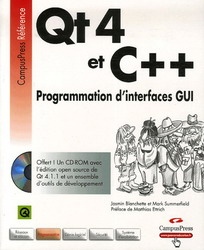
\includegraphics[scale=0.65]{Figures/coverCppProgrammingFrench.jpg}	
	\end{minipage}
	\hfill
	\begin{minipage}{0.48\linewidth}	
		\center	
		
\includegraphics[scale=0.25]{Figures/coverCppProgrammingFrench2.jpg}
	\end{minipage}
\end{frame}

\begin{frame}{Sur le web}
	\begin{itemize}
	\item<1-> En anglais
		\begin{itemize}
			\item Le site officiel de Nokia~: \texttt{\small doc.qt.nokia.com/}
			\item Un forum d'aide~: \texttt{\small www.qtforum.org}
		\end{itemize}
	\vspace{10 mm}
	\item<2-> En français
		\begin{itemize}
			\item<2-> Un forum d'aide: \texttt{\small www.developpez.net/forums/f376/c-cpp/bibliotheques/qt/}
			\item<2-> La documentation: \texttt{\small qt.developpez.com/doc/4.7/index/}
			\item<2-> Faq: \texttt{\small qt.developpez.com/faq/}
		\end{itemize}
	\end{itemize}
\end{frame}

\subsection{Survol des possibilités de Qt}
\begin{frame}	
	\begin{itemize}
	\item Les applications Qt possèdent un «look and feel» natif sur toutes les plateformes supportées
	\item<2-> Pour le portage entre les systèmes les plus connus (Linux, Windows, Mac OS X, \ldots) une simple recompilation est nécessaire
	\item<3-> Le portage peut aussi être effectué pour des environnements embarqués
	\item<4-> Qt intègre le support de la 3D grâce à des composants OpenGL
	\item<5-> Qt utilise l'Unicode et possède des composants dédiés à l'internationalisation (\textit{QString}, \textit{Qt Linguist})
	\end{itemize}
\end{frame}

\begin{frame}
	\begin{itemize}
	\item Qt permet l'utilisation de SGBD, indépendamment de la plateforme d'utilisation. Il est compatible notamment avec~: Oracle, SQLite, PostgreSQL, MySQL, \ldots
	\item<2-> Qt inclut un grand nombre de classes spécialisées pour un domaine~; il permet notamment la gestion directe du XML grâce à des parseurs SAX et DOM
	\item<3-> Qt inclue aussi des classes dédiées aux fonctionnalités réseaux et supporte les protocoles standard
	\item<4-> Qt fournit sa propre implémentation de la STL pour les compilateurs qui n'en seraient pas pourvus
	\item<5-> Pour faciliter la création des applications, le programme \textbf{Qt Designer} permet de créer rapidement les interfaces élémentaires
	\end{itemize}
\end{frame}

\begin{frame}
	\begin{itemize}
	\item Pour étendre Qt à de nouveaux composants et fonctionnalités, Qt propose un système d'extension (\textbf{Meta Object System}) et un compilateur (\textbf{Meta Object Compiler (MOC)}) qui permettent d'augmenter la puissance de la bibliothèque 
	\newline $\Rightarrow$ Mais cela empêche l'usage de l'héritage multiple
	\item<2-> Pour faciliter la création des Makefiles et autres fichiers de compilation, Qt propose l'outil \textbf{qmake} qui génère tous les fichiers nécessaires à compilation «propre»
	\end{itemize}
\end{frame}

%\part{Programmer avec Qt}
\section{La classe QObject et ses enfants}
\subsection{Le modèle objet de Qt}
\begin{frame}{Le modèle objet de Qt}
	\begin{itemize}
	\item<+-> Tous les \texttt{QObject}s s'organisent sous forme d'arbre
	\item<+-> Lors de la création d'un \texttt{QObject} avec un parent, le fils est ajouté à la liste \texttt{children()} du parent (destruction en cascade)
	\item<+-> La classe \texttt{QWidget} est la base de tous les composants affichables sur l'écran
		\begin{itemize}
			\item<+-> Un \texttt{QWidget} contenant tous ses enfants~: le fils d'un \texttt{QWidget} ne peut pas sortir des limites graphiques de son parent(i.e.: imbrication de widgets)
		\end{itemize}
	\item<+-> Les fonctions statiques \texttt{QObject::dumpObjectTree()} et \texttt{QObject::dumpObjectInfo()} sont souvent utiles au débogage de l'application
	\end{itemize}
\end{frame}

\begin{frame}{Arbre partielle des principaux objets}
	\begin{center}
		\tiny
		\begin{tikzpicture}
		[every node/.style={draw}]
			%level 0
			\node (QOBJECT) at (-1.5,0) {QObject};
									
			%level 1
			\node (QCOREAPPLICATION) at (-5,-1) {QCoreApplication};
			\node (QLAYOUT) at (-1.5,-1) {QLayout};
			\node (QWIDGET) at (3,-1) {QWidget};
									
			%level 2
			\node[visible on=<1>] (QAPPLICATION) at (-5,-2) {QApplication};
			\node[visible on=<2->,color=blue] (QAPPLICATION) at (-5,-2) {QApplication};
			\node (QVBOXLAYOUT) at (-3,-2) {QVBoxLayout};
			\node (QHBOXLAYOUT) at (0,-2) {QHBoxLayout};
			\node (QFRAME) at (2,-2) {QFrame};
			\node (QCOMBOBOX) at (4,-2) {QComboBox};
			
			%level 3
			\node (QLABEL) at (2,-3) {QLabel};
			
			%Lien
			\draw[->] (QOBJECT) -- (QCOREAPPLICATION) ; 
			\draw[->] (QOBJECT) -- (QLAYOUT) ;
			\draw[->] (QOBJECT) -- (QWIDGET) ;
			\draw[->] (QCOREAPPLICATION) -- (QAPPLICATION) ;
			\draw[->] (QLAYOUT) -- (QVBOXLAYOUT) ;
			\draw[->] (QLAYOUT) -- (QHBOXLAYOUT) ;
			\draw[->] (QWIDGET) -- (QFRAME) ;
			\draw[->] (QWIDGET) -- (QCOMBOBOX) ;
			\draw[->] (QFRAME) -- (QLABEL) ;
		\end{tikzpicture}
	\end{center}
	
	
	\begin{itemize}
	\item<2-> La classe \texttt{QApplication} permet interfacer l'application avec le système~: \alert{chaque application en possède une et une seule~!}
	\item<3-> \texttt{QApplication} implémente la boucle principale d'évènements
	\item<4-> L'objet \texttt{QApplication} a besoin d'un composant principal sur lequel renvoyer les évènements capturés
	\end{itemize}
\end{frame}
\begin{frame}{Le modèle objet de Qt}	
	\begin{itemize}
	\item Qt est basé autour du modèle d'objet de Qt
	\item<2-> Son architecture est entièrement fondée sur la classe \texttt{QObject} et de l'outil \textbf{moc}
	\item<3-> En dérivant des classes de \texttt{QObject}, un certain nombre d'avantages sont hérités~:
		\begin{itemize}
		\item<4-> Gestion facile de la mémoire
		\item<5-> Signaux et Slots
		\item<6-> Propriétés
		\item<7-> Introspection (capacité du programme à examiner son état)
		\end{itemize}
	\item<8-> Qt, c'est uniquement du \texttt{C++} standard avec quelques macros (d'où la portabilité)
	\end{itemize}
\end{frame}

\subsection{La gestion «facile» de la mémoire}
\begin{frame}{La gestion «facile» de la mémoire}
	
	\begin{itemize}
	\item En créant une instance d'une classe dérivée de \texttt{QObject}, il est possible de passer un pointeur vers un objet parent au constructeur
	\item<2-> Quand un parent est supprimé, ses enfants sont supprimés aussi
	\item<3-> \alert{Il ne faut donc pas détruire manuellement les enfants !}
	\item<4-> \alert{Le <<top level widget>> ne doit pas être instancié par \texttt{new} !}
	\end{itemize}
\end{frame}

\begin{frame}
	\begin{exampleblock}{Exemple}
		\lstinputlisting[style=customcpp]{code/verboseObject.cpp}
	\end{exampleblock}
\end{frame}


\begin{frame}
	\begin{exampleblock}{}
		\begin{minipage}{0.48\linewidth}
			\lstinputlisting[style=customcpp]{code/mainVerboseObject.cpp}
		\end{minipage}
		\hfill
		\begin{minipage}{0.48\linewidth}
			\begin{center}
				\tiny
				\begin{tikzpicture}
				[every node/.style={circle,draw}]
				\node[opacity=0] (NONE) at (0,4.5) {};
					%level 0
					\node[visible on=<1->] (TOP) at (0,0) {$TOP$};
											
					%level 1
					\node[visible on=<2->] (X) at (-1,-1) {$X$};
											
					%level 2
					\node[visible on=<3->] (Y) at (1,-1) {$Y$};
					
					%level 3
					\node[visible on=<4->] (Z) at (-1,-2) {$Z$};
					
					%Lien
					\draw[visible on=<2->,->] (TOP) -- (X) ; 
					\draw[visible on=<3->,->] (TOP) -- (Y) ;
					\draw[visible on=<4->,->] (X) -- (Z) ;
				\end{tikzpicture}
			\end{center}
		\end{minipage}
	\end{exampleblock}
\end{frame}

\begin{frame}
	\begin{exampleblock}{}
		\begin{minipage}{0.48\linewidth}
			\begin{tabbing}
				\$ ./mem\\
				Created\\
				Created\\
				Created\\
				Created\\
				Do stuff: top\\
				Do stuff: x\\
				Do stuff: y\\
				Do stuff: z\\
				Deleted: top\\
				Deleted: x\\
				\alert{Deleted: z}\\
				Deleted: y\\	
			\end{tabbing}	
		\end{minipage}
		\hfill
		\begin{minipage}{0.48\linewidth}
			\begin{center}
				\tiny
				\begin{tikzpicture}
				[every node/.style={circle,draw}]
					%level 0
					\node[visible on=<1>] (TOP) at (0,0) {$TOP$};
					\node[visible on=<2->, cross out, color=red] (TOP) at (0,0) {$TOP$};
											
					%level 1
					\node[visible on=<1-2>] (X) at (-1,-1) {$X$};
					\node[visible on=<3->, cross out, color=red] (X) at (-1,-1) {$X$};
											
					%level 2
					\node[visible on=<1-4>] (Y) at (1,-1) {$Y$};
					\node[visible on=<5->, cross out, color=red] (Y) at (1,-1) {$Y$};
					
					%level 3
					\node[visible on=<1-3>] (Z) at (-1,-2) {$Z$};
					\node[visible on=<4->, cross out, color=red] (Z) at (-1,-2) {$Z$};
					
					%Lien
					\draw[visible on=<1->,->] (TOP) -- (X) ; 
					\draw[visible on=<1->,->] (TOP) -- (Y) ;
					\draw[visible on=<1->,->] (X) -- (Z) ;
				\end{tikzpicture}
			\end{center}
				\begin{itemize}
				\item<6-> Si la référence du parent est enlevée de \texttt{x} et de \texttt{y}, une fuite de mémoire se produit
				\end{itemize}
		\end{minipage}
	\end{exampleblock}
\end{frame}

\subsection{QWidgets}
\begin{frame}{QWidgets}
	\begin{center}
		\tiny
		\begin{tikzpicture}
		[every node/.style={draw}]
			%level 0
			\node (QOBJECT) at (-1.5,0) {QObject};
									
			%level 1
			\node (QCOREAPPLICATION) at (-5,-1) {QCoreApplication};
			\node[visible on=<1>] (QLAYOUT) at (-1.5,-1) {QLayout};
			\node[visible on=<2->,color=red] (QLAYOUT) at (-1.5,-1) {QLayout};
			\node[color=blue] (QWIDGET) at (3,-1) {QWidget};
									
			%level 2
			\node (QAPPLICATION) at (-5,-2) {QApplication};
			\node (QVBOXLAYOUT) at (-3,-2) {QVBoxLayout};
			\node (QHBOXLAYOUT) at (0,-2) {QHBoxLayout};
			\node (QFRAME) at (2,-2) {QFrame};
			\node (QCOMBOBOX) at (4,-2) {QComboBox};
			
			%level 3
			\node (QLABEL) at (2,-3) {QLabel};
			
			%Lien
			\draw[dotted,visible on=<2->,color=red] (QLAYOUT) -- (QWIDGET) ;
			\draw[->] (QOBJECT) -- (QCOREAPPLICATION) ; 
			\draw[->] (QOBJECT) -- (QLAYOUT) ;
			\draw[->] (QOBJECT) -- (QWIDGET) ;
			\draw[->] (QCOREAPPLICATION) -- (QAPPLICATION) ;
			\draw[->] (QLAYOUT) -- (QVBOXLAYOUT) ;
			\draw[->] (QLAYOUT) -- (QHBOXLAYOUT) ;
			\draw[->] (QWIDGET) -- (QFRAME) ;
			\draw[->] (QWIDGET) -- (QCOMBOBOX) ;
			\draw[->] (QFRAME) -- (QLABEL) ;
		\end{tikzpicture}
	\end{center}
	\begin{alertblock}{Dévellopeur android, attention}<2->
		En Qt, un widget n'est pas un layout et un layout n'est pas un widget.
	\end{alertblock}

\end{frame}

\begin{frame}
	\begin{itemize}
	\item Qt fournit un panel complet de widgets
	\item<2-> Tout widget adapté (personnalisé) est créé par héritage d'un widget existant
		\begin{itemize}
			\item<3-> Pour créer son propre widget <<from scratch>>, il suffit d'hériter de \texttt{QWidget}
		\end{itemize}
	\item<4-> Un widget peut contenir plusieurs widgets fils~:
		\begin{itemize}
			\item<5-> Les widgets fils ne peuvent s'afficher en dehors du parent 
		\end{itemize}
	\item<6-> Un widget sans parent est un «top-level» (racine) widget. \color{red} Le top-level widget ne devrait pas être un pointeur.\color{black}
	\item<7-> Un widget peut être positionné de manière automatique, grâce aux «layout managers» (gestionnaire de placement) ou manuellement. \color{red} Attention: Widget $ \not= $ Layout  \color{black}
	\item<8-> Quand un widget est désactivé, caché ou détruit, la même action est appliquée récursivement à ses enfants
	\end{itemize}
\end{frame}

\begin{frame}
	\begin{exampleblock}{Le <<hello world!>>}
		\lstinputlisting[style=customcpp]{code/helloWorld.cpp}
	\end{exampleblock}
	\visible<2->{\centerline{\pgfimage[width=2.5cm]{Figures/capture_helloworld}}}
\end{frame}

\begin{frame}[fragile]
	\begin{exampleblock}{}
	\begin{itemize}
		\item L'application créée sa propre fenêtre et appelle la boucle infinie de capture d'évènements
		\begin{itemize}
		\item<2-> La boucle de capture des évènements est incluse dans l'appel à \texttt{app.exec()}
		\end{itemize}
	\item<3-> Les évènements sont capturés par l'application, il ne reste qu'à leur associer des réactions aux widgets
	\item<4-> Remarques sur les widgets~:
		\begin{itemize}
		\item<5-> Chaque classe commence par un 'Q'
		\item<6-> Pour chaque classe correspond un fichier de déclarations à inclure
		\item<7-> Conséquence~: la liste des fichiers à inclure augmente rapidement \ldots
		\item<8-> \ldots  Ou bien vous pouvez inclure le fichier qui inclut tout les fichiers de déclaration ( \verb+#include <QtGui/QtGui>+ ) $ \Rightarrow $ Compilation plus longue.
		\end{itemize}
	\end{itemize}
	\end{exampleblock}
\end{frame}

\begin{frame}
	\frametitle{Les widgets utilisateur courants <1>}
	
	\begin{itemize}
	\item Pour concevoir une interface graphique, il faut connaître les widgets courants de la librairie graphique utilisée~:
	\end{itemize}
	
	\centerline{\begin{tabular}{ll}
	\multicolumn{1}{c}{\underline{Widget}} & \multicolumn{1}{c}{\underline{Description}} \\
	\ttfamily QLabel & Affiche du texte et des images\\
	\ttfamily QCheckBox & Une boîte à cocher avec une étiquette\\
	\ttfamily QLCDNumber & Afficheur digital\\
	\ttfamily QLineEdit & Une simple ligne d'édition\\
	\ttfamily QTextEdit & Version plus riche, multi-ligne du widget précédent\\
	\ttfamily QListView & Une liste d'éléments à une colonne (peut être «scrollée»)\\
	\ttfamily QMenu & Tous les types de menus (normaux, pop up)\\
	\ttfamily QProgressBar & Barre de progression pour les opérations longues\\
	\ttfamily QPushButton & Bouton à cliquer (avec du texte ou une image)\\
	\end{tabular}}
\end{frame}

% ICI

\begin{frame}
	\frametitle{Les widgets utilisateur courants}
	
	\centerline{\begin{tabular}{ll}
	\multicolumn{1}{c}{\underline{Widget}} & \multicolumn{1}{c}{\underline{Description}} \\
	\ttfamily QRadioButton & Bouton radio (on/off en cercle) avec étiquette\\
	\ttfamily QScrollBar & Barre de défilement horizontale ou verticale\\
	\ttfamily QSlider & Barre de niveau horizontale ou verticale\\
	\ttfamily QSpinBox & Boîte de saisie avec des flèches haut/bas\\
	\ttfamily QToolButton & Un bouton à cliquer formaté pour les barres d'outils\\
	\ttfamily QWhatsThis & Fournit une fenêtre d'informations sur les widgets\\
	\end{tabular}}
\end{frame}

\begin{frame}
	\frametitle{Les widgets utilisés pour grouper des widgets}
	\centerline{\begin{tabular}{ll}
	\multicolumn{1}{c}{\underline{Widget}} & \multicolumn{1}{c}{\underline{Description}} \\
	\ttfamily QFrame & Classe de base pour les widgets avec frames\\
	\ttfamily QGroupBox & Groupe horizontalement ou verticalement \\
		& les éléments dans un cadre (ligne)\\
	\ttfamily QHBoxLayout & Groupe horizontalement les éléments sans frame\\
	\ttfamily QVBoxLayout & Groupe verticalement les éléments sans frame\\
	\ttfamily QMenuBar & Barre contenant les menus\\
	\ttfamily QToolBar & Barre contenant des boutons spécifiques\\
	\ttfamily QMainWindow & Grande fenêtre principale plus menus et barre de boutons\\
	\ttfamily QDialog & Frame qui apparait en popup contenant d'autres widgets\\
	\end{tabular}}
\end{frame}

\subsection{QLayouts}
\begin{frame}
	\begin{center}
		\tiny
		\begin{tikzpicture}
		[every node/.style={draw}]
			%level 0
			\node (QOBJECT) at (-1.5,0) {QObject};
									
			%level 1
			\node (QCOREAPPLICATION) at (-5,-1) {QCoreApplication};
			\node[color=blue] (QLAYOUT) at (-1.5,-1) {QLayout};
			\node[visible on=<1>] (QWIDGET) at (3,-1) {QWidget};
			\node[visible on=<2->, color=red] (QWIDGET) at (3,-1) {QWidget};
									
			%level 2
			\node (QAPPLICATION) at (-5,-2) {QApplication};
			\node (QVBOXLAYOUT) at (-3,-2) {QVBoxLayout};
			\node (QHBOXLAYOUT) at (0,-2) {QHBoxLayout};
			\node (QFRAME) at (2,-2) {QFrame};
			\node (QCOMBOBOX) at (4,-2) {QComboBox};
			
			%level 3
			\node (QLABEL) at (2,-3) {QLabel};
			
			%Lien
			\draw[dotted,visible on=<2->,color=red] (QLAYOUT) -- (QWIDGET) ;
			\draw[->] (QOBJECT) -- (QCOREAPPLICATION) ; 
			\draw[->] (QOBJECT) -- (QLAYOUT) ;
			\draw[->] (QOBJECT) -- (QWIDGET) ;
			\draw[->] (QCOREAPPLICATION) -- (QAPPLICATION) ;
			\draw[->] (QLAYOUT) -- (QVBOXLAYOUT) ;
			\draw[->] (QLAYOUT) -- (QHBOXLAYOUT) ;
			\draw[->] (QWIDGET) -- (QFRAME) ;
			\draw[->] (QWIDGET) -- (QCOMBOBOX) ;
			\draw[->] (QFRAME) -- (QLABEL) ;
		\end{tikzpicture}
	\end{center}
	\begin{alertblock}{Dévellopeur android, attention}<2->
		En Qt, un widget n'est pas un layout et un layout n'est pas un widget.
	\end{alertblock}
\end{frame}


\begin{frame}{Gestionnaire de placement - « Layout Manager »}
	\begin{itemize}
	\item Un des problèmes lors de la conception d'une interface graphique concerne le placements des widgets~:
		\begin{itemize}
		\item<2-> Le placement initial
		\item<3-> Le comportement lorsque la fenêtre s'agrandit ou se rétrécit
		\end{itemize}
	\item<4-> Pour éviter ces problèmes~: utiliser un «Layout Manager»
	\item<5-> Qt propose deux types de layout managers~:
		\begin{itemize}
		\item<6-> \texttt{QBoxLayout} qui range les widgets soit verticalement (\texttt{QVBoxLayout}) soit horizontalement (\texttt{QHBoxLayout})
		\item<7-> \texttt{QGridLayout} qui range les widgets comme dans un tableau
		\end{itemize}
	\end{itemize}
	\begin{alertblock}{Attention}<8->
	La classe \texttt{QBox} permet de ranger les widgets, mais lors d'un agrandissement ou rétrécissement de la fenêtre, les widgets ne sont pas replacés.
	\end{alertblock}
\end{frame}

\begin{frame}{Les «~\texttt{QBoxLayout}~» }
	\begin{itemize}
	\item Reçoit la place que prend le widget parent et le divise en petit carrés destinés à contenir les widgets à placer
	\item<2-> \texttt{QBoxLayout} est très rarement utilisé, on utilise plutôt les classes \texttt{QHBoxLayout} et \texttt{QVBoxLayout} qui en héritent directement
	\item<3-> Les widgets sont rangés selon l'ordre dans lequel ils sont ajoutés au layout
	\item<4-> Il est possible de passer au constructeur un entier qui initialisera le nombre de cases prévues au départ
	\item<5-> Les layouts peuvent être imbriqués grâce à la méthode \texttt{addLayout} ou encore en l'initialisant avec un layout comme parent
	\end{itemize}
\end{frame}

\begin{frame}{Les «~\texttt{QBoxLayout}~» }
	\begin{exampleblock}{}
		\lstinputlisting[style=customcpp]{code/hBoxLayout.cpp}
		\visible<2->{\hspace*{7cm}\smash{
			\begin{minipage}[t]{4cm}
				\pgfimage[width=3cm]{Figures/capture_boxlayout}
		\end{minipage}}}\\
	\end{exampleblock}
\end{frame}

\begin{frame}
	\frametitle{Le «~\texttt{QGridLayout}~»}
	
	\begin{itemize}
	\item Un \texttt{QGridLayout} divise l'espace comme un tableau où chaque cellule est identifiable par son numéro de ligne et de colonne (débutant à 0)
	\item<2-> Le nombre de lignes et de colonnes s'adapte en fonction des widgets placés
	\item<3-> Il existe plusieurs constructeurs permettant notamment de définir initialement le nombre de lignes et de colonnes
	\item<4-> Les cases vides sont acceptées
	\item<5-> La largeur minimale d'une colonne peut être définie avec~: \texttt{setColumnMinimumWidth( int col, int space )}
	\item<6-> La hauteur minimale d'une ligne peut être définie avec~: \texttt{setRowMinimumHeight( int row, int space )}
	\end{itemize}
\end{frame}

\begin{frame}
	\begin{exampleblock}{}
		\lstinputlisting[style=customcpp]{code/gridBoxLayout.cpp}
 		\visible<2->{\hspace*{7.5cm}\smash{
			\begin{minipage}[t]{4cm}
				\pgfimage[width=3cm]{Figures/capture_gridlayout}
			\end{minipage}}}
	\end{exampleblock}
\end{frame}

\begin{frame}
	\begin{block}{Les propriétés des widgets utilisées par le layout manager}
	\begin{itemize}
	\item Les widgets intègrent des propriétés qui déterminent leur comportement lors de leur placement et dimensionnement
		\begin{itemize}
		\item<2-> Exemple~: \textit{la taille des boutons}\newline
		\hspace*{2cm}\pgfimage[width=2.5cm]{Figures/capture_boutonslayout}
		\end{itemize}
	\item<3-> Les propriétés de redimensionnement (taille) sont personnalisables grâce à la classe \texttt{QSizePolicy}
	\item<4-> Les espacements entre widgets peuvent être modifiés~:
		\begin{itemize}
		\item<5-> Soit en spécifiant des marges dans les layouts (\texttt{setMargin(int)} et \texttt{setSpacing(int)})
		\item<6-> Soit en utilisant ponctuellement les méthodes \texttt{addSpacing(int)} et \texttt{insertSpacing(int,int)} ajoutant un espace dans le layout
		\end{itemize}
	\end{itemize}
	\end{block}
\end{frame}

\begin{frame}
	\begin{block}{Les propriétés des widgets utilisées par le layout manager}
	\begin{itemize}
	\item Lorsque l'on souhaite que ce soit les espacements qui varient et non pas la taille des widgets on peut utiliser des élastiques
	\item<2-> Les méthodes \texttt{addStretch(int)} et \texttt{insertStretch(int,int)}  permettent d'ajouter un élastique à un widget avec un poids passé en paramètre
	\item<3-> Toutes les commandes d'élastiques vues s'adaptent aussi sur les \texttt{QGridLayout} en utilisant les méthodes~: {\ttfamily setRowStretch, \textrm{et} setColumnStretch}
	\end{itemize}
	
	\visible<4->{\centerline{\pgfimage[width=4cm]{Figures/capture_boxstretchlayout}}}
	\end{block}
\end{frame}

\subsection{Les signaux et les slots}

\begin{frame}
	\begin{itemize}
	\item Toute application (graphique) doit permettre de traiter les évènements
		\begin{itemize}
		\item<2-> Exemple~: le clic sur un bouton déclenche la fermeture de l'application
		\end{itemize}
	\item<3-> Pour cela, Trolltech a créé pour Qt une solution appelée «~signals and slots~», \color{red}indépendante d'une GUI \color{black}
	\item<4-> Les signaux et slots sont des mécanismes génériques de communication inter-objets
	\item<5-> Ils sont utilisés pour remplacer les «~anciens~» mécanismes de «~callbacks~»~:
		\begin{itemize}
		\item<6-> Un callback consiste en un pointeur sur une fonction passé à un bouton (par exemple) qui est appelée lorsque que le bouton est cliqué
		\item<7-> Aucune vérification du typage par le compilateur~!
		\item<8-> Il est difficile de développer des classes génériques indépendantes des évènements qu'elles traitent
		\end{itemize}
	\end{itemize}
\end{frame}

\begin{frame}{Fonctionnement}
	
	\centerline{\pgfimage[width=7cm]{Figures/abstract-connections}}
\end{frame}

\begin{frame}{Fonctionnement}

	\begin{itemize}
	\item Un signal est émis quand un évènement se produit
	\item<2-> Un slot est une méthode (ou fonction) appelée en réponse à un signal particulier
	\item<3-> Qt intègre un grand nombre de slots prédéfinis, mais il est possible de créer ses propres slots (et signaux)
	\item<4-> Le mécanisme des signaux et slots est «~type-safe~», et les erreurs de typage sont reportées comme avertissement lors de la compilation
	\item<5-> La méthode \texttt{QObject::connect} permet d'associer un signal à un slot
	\item<6-> Les connexions peuvent être ajoutées et enlevées à n'importe quel moment durant l'exécution
	\end{itemize}
\end{frame}

\begin{frame}{Fonctionnement}

	\begin{itemize}
	\item Toutes les classes héritant de \texttt{QObject} peuvent contenir des signaux et des slots
	\item<2-> Il est possible de connecter un signal à plusieurs slots, et plusieurs signaux à un seul slot~:
	\end{itemize}

	\visible<3->{\centerline{\pgfimage[width=12cm]{Figures/concrete-connections}}}
\end{frame}

\begin{frame}{Exemple}
	\begin{exampleblock}{Quitter une application}
		\lstinputlisting[style=customcpp]{code/signal.cpp}
	\end{exampleblock}
\end{frame}

\begin{frame}
	\frametitle{Les signaux}
	
	\begin{itemize}
	\item Les signaux sont émis par un objet lorsque son état change
	\item<2-> Seules les classes définissant un signal peuvent émettre \alert{ce} signal
	
	\begin{alertblock}<3->{Remarque}
	Les signaux sont déclarés, mais ils ne sont jamais implémentés dans le .cpp~! Leur implémentation est générée automatiquement par le moc (Meta Object Compiler).
	\end{alertblock}
	
	\item<4-> Le concepteur peut émettre un signal particulier grâce au mot clef \texttt{emit}
	\item<5-> Quand un signal est émis, les slots connectés sont exécutés immédiatement
	\item<6-> Si plusieurs slots sont connectés à un signal, leur ordre d'exécution est réalisé dans l'ordre de la déclaration de leurs connexions(\texttt{QObject::connect()}).
	\end{itemize}
\end{frame}

\begin{frame}
	\frametitle{Les slots}
	
	\begin{itemize}
	\item Un slot est appelé dès que le signal connecté est émis
	\item<2-> Comme les slots sont des méthodes normales, ils possèdent les mêmes droits que d'autres méthodes classiques
	\item<3-> Comme les autres attributs d'une classe, les slots peuvent être déclarés \texttt{private}, \texttt{protected} et \texttt{public}
	\item<4-> Les slots peuvent aussi être virtuels (\texttt{virtual})
	\item<5-> Les slots sont plus lents que les fonctions de «~callback~», mais la différence n'est pas décelable par l'utilisateur
	\end{itemize}
\end{frame}

\begin{frame}{Créer ses propres signaux et slots}
	
	\begin{itemize}
	\item Les signaux et slots définis dans Qt ne sont pas suffisants
	\item<2-> Qt propose des solutions pour définir ses propres signaux et slots, mais attention :
		\begin{itemize}
		\item<3-> Il n'est pas possible de définir une classe qui ne contient que des slots ou des signaux
		\item<4-> Les signaux et slots ne peuvent être déclarés que dans des classes qui héritent de \texttt{QObject}
		\item<5-> Dans toute classe définissant des signaux ou slots, il faut placer la macro \texttt{Q\_OBJECT}
		\item<6-> Les paramètres par défaut ne sont pas utilisables pour les signaux et les slots
		\end{itemize}
	\end{itemize}
\end{frame}
	
\begin{frame}{Créer ses propres signaux et slots}
	
	\begin{block}{Definition}
		\lstinputlisting[style=customcpp]{code/myClass.cpp}
	\end{block}
\end{frame}

\begin{frame}{Créer ses propres signaux et slots}
	
	\begin{itemize}
	\item Cette classe est différente d'une classe C++ standard
		\begin{itemize}
		\item<2-> Elle hérite obligatoirement de \texttt{QObject}
		\item<3-> Elle fait appel à la macro \texttt{Q\_OBJECT}
		\item<4-> De nouveaux mots clefs apparaissent~: {\ttfamily signals, private slots, \ldots}
		\item<5-> Les méthodes définies dans les sections slots retournent \alert{obligatoirement} le type void
		\end{itemize}
	\item<6-> Ce type de classe ne peut pas être compilé avec le compilateur C++ habituel~:
		\begin{itemize}
		\item<7-> Il est nécessaire d'utiliser en premier lieu le compilateur \texttt{moc}
		\item<8-> \texttt{moc} remplace tous les mots clefs spécifiques par des commandes et appels C++ implémentant le comportement voulu de l'objet
		\end{itemize}
	\end{itemize}
\end{frame}
	
\begin{frame}{Créer ses propres signaux et slots}
	\framesubtitle{Exemple}
	\begin{exampleblock}{Fichier .h}
		\lstinputlisting[style=customcpp]{code/foo.h}
	\end{exampleblock}
\end{frame}

\begin{frame}{Créer ses propres signaux et slots}
	\framesubtitle{Exemple}
	\begin{exampleblock}{Fichier .cpp}
		\lstinputlisting[style=customcpp]{code/foo.cpp}
	\end{exampleblock}
\end{frame}
	
\begin{frame}{Créer ses propres signaux et slots}
	\framesubtitle{Exemple}
	\begin{exampleblock}{main.cpp}
		\lstinputlisting[style=customcpp]{code/fooMain.cpp}
	\end{exampleblock}
\end{frame}
	
\section{Développer avec et pour Qt}
\subsection{Présentation des outils}
\begin{frame}
	\begin{itemize}
	\item<+-> Qt est fourni avec un grand nombre d'outils graphiques ou en ligne de commande pour accélérer les phases de développement~:
		\begin{itemize}
		\item<+-> \textbf{qtconfig} - permet de modifier des paramètres communs à toutes les applications \texttt{Qt}
		\item<+-> \textbf{Qt Designer} - permettant de dessiner les widgets en mode graphique
		\item<+-> \textbf{Qt Linguist, lupdate et lrelease} - utilisés pour la traduction des messages de l'application développée
		\item<+-> \textbf{Qt Assistant} - un outil graphique d'aide sur Qt
		\item<+-> \textbf{qmake} - chargé de créer des \textit{Makefiles} appropriés
		\item<+-> \textbf{qembed} - permettant la conversion de fichiers images (par exemple) en code C++
		\item<+-> \textbf{rcc} - permet d'incorporer des données extérieures (icônes, images, \ldots) à la compilation
		\item<+-> \textbf{moc} - le Meta Object Compiler
		\item<+-> \textbf{uic} - le User Interface Compiler
		\end{itemize}
	\end{itemize}
\end{frame}

\subsection{Les fonctionnalités de déboggage}
\begin{frame}
	\begin{itemize}
	\item Messages d'avertissements~:
		\begin{itemize}
		\item<2-> \texttt{qDebug( const char * msg, ... )} qui affiche un message de déboggage
		\item<3-> \texttt{qWarning( const char * msg, ... )} qui affiche un avertissement
		\item<4-> \texttt{qFatal( const char * msg, ... )} qui affiche un message d'erreur puis quitte l'application
		\end{itemize}
	\item<5-> Toutes ces fonctions affichent leur message sur la sortie d'erreur standard (sous Unix)~: \texttt{stderr}
	\item<6-> Il est aussi possible de rediriger et reformater les sorties de ces fonctions grâce à l'utilisation de \texttt{qInstallMsgHandler}
	\end{itemize}
\end{frame}

\begin{frame}
	\begin{exampleblock}{Exemple}
		\lstinputlisting[style=customcpp]{code/deboggage.cpp}
	\end{exampleblock}

	\begin{itemize}
	\item<2-> \texttt{qInstallMsgHandler(0)} restaure le traitement initial
	\end{itemize}
\end{frame}

\begin{frame}
	\begin{itemize}
	\item Qt fournit aussi des macros~: \texttt{Q\_ASSERT(b)} et \texttt{Q\_CHECK\_PTR(p)}
		\begin{itemize}
		\item<2-> \texttt{Q\_ASSERT(b)} ou \texttt{b} est un booléen écrit un assert si \texttt{b} est faux
		\item<3-> \texttt{Q\_CHECK\_PTR(p)} ou \texttt{p} est un pointeur écrit un avertissement si \texttt{p} est nul
		\end{itemize}
	\end{itemize}

	\begin{exampleblock}{Exemple}<4->
		\lstinputlisting[style=customcpp]{code/deboggage2.cpp}
	\end{exampleblock}
\end{frame}

\subsection{Qt Assistant et Qt Linguist}
\begin{frame}
	\alt<1>{\centerline{\pgfimage[width=6.5cm]{Figures/capture_assistant}}}%
		{\centerline{\pgfimage[width=7cm]{Figures/capture_linguist}}}

	\begin{itemize}
	\item Qt Assistant est un outil d'aide pour la documentation de Qt
	\item<2-> Qt Linguist et ses petits outils (\texttt{lrelease} et \texttt{lupdate}) permettent de traduire simplement le texte d'une application Qt
	\end{itemize}
\end{frame}


\begin{frame}
	\begin{enumerate}\itshape
	\item Premièrement, il faut créer un fichier projet.pro contenant la liste des fichiers de langue à traiter
	\item<2-> Puis il faut utiliser l'outil \texttt{lupdate} qui extrait du code source le texte à traduire
	\item<3-> Ensuite, à l'aide Qt linguist, traduire le texte
	\item<4-> Enfin exécuter la commande \texttt{lrelease} qui génère les fichiers traduits prêts à l'emploi
	\end{enumerate}
\end{frame}

\begin{frame}
\begin{exampleblock}{Exemple traduc.cpp}
	\lstinputlisting[style=customcpp]{code/traduc.cpp}
\end{exampleblock}

\begin{exampleblock}{Exemple traduc.pro}<2->
	\lstinputlisting{code/traduc.pro}
\end{exampleblock}
\end{frame}

\subsection{Qt Designer, UI Compiler}
\begin{frame}
	\centerline{\pgfimage[width=5.4cm]{Figures/capture_designer}}

	\begin{itemize}
	\item Qt Designer permet de dessiner à l'aide de la souris l'interface graphique de l'application
	\item<2-> Le résultat est sauvegardé dans un fichier xml à l'extension .ui
	\item<3-> Le User Interface Compiler (uic) transforme les fichiers .ui généré par Qt designer pour les transformer en fichiers sources ou entêtes C++
	\end{itemize}
\end{frame}

\subsection{le Meta Object Compiler (moc)}
\begin{frame}
	\begin{itemize}
	\item Le Meta Object Compiler (moc) permet de pré-compiler les extensions développées pour Qt
	\item<2-> Il pré-compile tout fichier contenant des instructions du «~meta object system~», i.e~:
		\begin{itemize}
		\item<3-> \alert{Le fichier doit contenir la macro \texttt{Q\_OBJECT}}
		\item<4-> Possibilité d'ajouter des slots ou des signaux aux classes héritant de QObject
		\item<5-> Possibilité d'ajouter des propriétés aux objets aux classes héritant de QObject
		\item<6-> Possibilité d'utiliser \texttt{tr()} (internationalisation) directement sur la classe \texttt{QObject}
		\item<7-> Utilisation des macros~: {\ttfamily Q\_PROPERTY, Q\_ENUMS, Q\_CLASSINFO, Q\_INTERFACES et Q\_FLAGS}
		\item<8-> \ldots
		\end{itemize}
	\end{itemize}
\end{frame}

\begin{frame}
	\begin{itemize}
	\item Le résultat produit par le moc doit être lié avec le reste des fichiers compilés pour produire le programme exécutable
	\item<2-> \textbf{Méthode A~:} les instructions du «~meta object system~» se trouve dans un fichier myclass.h. Le résultat de l'exécution du moc doit être écrit dans un fichier nommé moc\_myclass.cpp qui devra être compilé et lié comme d'habitude
	\item<3-> \textbf{Méthode B~:} les instructions du «~meta object system~» se trouve dans un fichier myclass.cpp. Le résultat de l'exécution du moc doit être écrit dans un fichier nommé myclass.moc. Ce fichier doit être inclus à la fin du fichier myclass.cpp (\texttt{\#include "myclass.moc"}) qui sera compilé comme d'habitude
	\item<4-> \alert{La méthode normale est bien sûr la méthode A !}
	\item<5-> Il est conseillé de lire le manuel du moc car il existe des limitations et des cas particuliers
	\end{itemize}
\end{frame}

\subsection{qmake}
\begin{frame}
	\begin{itemize}
	\item qmake est un outil permettant d'automatiser la génération des makefiles pour des applications Qt~:
		\begin{itemize}
		\item Prise en compte du moc, du uic et d'autres spécificités Qt
		\end{itemize}
	\item<2-> qmake utilise un fichier d'information (.pro) pour générer les makefiles appropriés
	\end{itemize}
		
	\begin{exampleblock}<3->{Fichier monprojet.pro}
		\lstinputlisting{code/monProjet.pro}
	\end{exampleblock}
	
	\begin{itemize}
	\item<4-> Exécution~: \texttt{qmake -o Makefile monprojet.pro}
	\end{itemize}
\end{frame}

\begin{frame}
	\begin{exampleblock}{Fichier monprojet.pro}
		\lstinputlisting{code/monProjet.pro}
	\end{exampleblock}
		
	\begin{itemize}
	\item \texttt{qt} indique à qmake que l'application est construite pour Qt (ajout des librairies et des répertoires d'includes)
	\item<2-> \texttt{warn\_on} indique à qmake que les warnings du compilateur seront affichés
	\item<3-> \texttt{release} indique à qmake que l'application compilée est dédiée à la diffusion. Le programmeur peut remplacer \texttt{release} par \texttt{debug}
	\item<4-> Il faut toujours utiliser le \texttt{+=} pour la partie \texttt{CONFIG} car il ne faut pas effacer les options déjà existantes
	\end{itemize}
\end{frame}

\begin{frame}
	\begin{itemize}
	\item qmake permet d'ajouter des parties spécifiques à chaque plateforme et de tester certaines conditions comme l'existance d'un fichier
	\end{itemize}

\begin{exampleblock}{Fichier hello.pro}<2->
	\lstinputlisting{code/hello.pro}
\end{exampleblock}
\end{frame}


\section{Redéfinition de widgets et d'évènements avec Qt}
\subsection{Introduction}

\begin{frame}
	\frametitle{Quand les slots et signaux ne suffisent plus}
	
	\begin{itemize}
	 \item<+-> Lorsque l'on veut créer/étendre un widget, la solution des signaux et slots est parfois insuffisante
	 \item<+-> Il faut gérer les évènements plus finement, au plus près du widget de manière à redéfinir son comportement
	 \item<+-> Dans ce but, Qt permet de manipuler des objets issus de sous-classes de la classe \texttt{QEvent}
	 \item<+-> Les évènements peuvent être reçus et gérer par tout objet issu d'une sous-classe de \texttt{QObject}, mais sont intéressant surtout dans le cas des widgets
	\end{itemize}
\end{frame}

\begin{frame}
	\frametitle{Comment sont reçus les évènements}
	
	\begin{itemize}
	 \item<+-> Quand un évènement est reçu, Qt crée un objet instance de la sous-classe appropriée de \texttt{QEvent}
	 \item<+-> Cet objet est ensuite passé au widget destination par l'appel à sa méthode \texttt{event()}
	 \item<+-> Cette méthode ne traite pas directement l'évènement, mais exécute la méthode de gestion appropriée en fonction du type de l'évènement reçu
	 \item<+-> Elle renvoie une réponse rendant compte du traitement ou du refus de l'évènement
	 \item<+-> Certains évènements comme \texttt{QMouseEvent} et \texttt{QKeyEvent} sont émis par le système, d'autres comme \texttt{QTimerEvent} proviennent d'autres sources ou programmes
	\end{itemize}
\end{frame}

\begin{frame}
	\frametitle{Les types d'évènements}
	
	\begin{itemize}
	 \item<+-> La plupart des évènements ont leur classe de traitement~: \texttt{QResizeEvent}, \texttt{QPaintEvent}, \texttt{QMouseEvent}, \texttt{QKeyEvent}, \texttt{QCloseEvent}, \ldots
	 \item<+-> Chaque sous-classe comporte des fonctions spécifiques adaptées à l'évènement traitée~: \texttt{QResizeEvent} comprend les méthodes \texttt{size()} et \texttt{oldSize()} pour permettre aux widgets de connaître l'évolution de leur taille
	 \item<+-> Certaines classes comme \texttt{QMouseEvent} peuvent gérer plusieurs évènements (le click, le double click, \ldots)
	\end{itemize}
\end{frame}

\subsection{Gestion des évènements}
\begin{frame}
	\begin{itemize}
	 \item<+-> Habituellement, un évènement est traité par l'appel d'une méthode virtuelle~: \texttt{QPaintEvent} est géré lors de l'appel à la méthode \texttt{paintEvent()}
	 \item<+-> Cette méthode est responsable du traitement de l'évènement, toutefois, il est parfois nécessaire de faire appel aux classes de bases pour finir la gestion d'un évènement
	\end{itemize}
	
\begin{exampleblock}{Exemple}<+->
	\lstinputlisting[style=customcpp]{code/checkBox.cpp}
\end{exampleblock}
\end{frame}

\begin{frame}
	\begin{itemize}
	 \item<+-> Il arrive qu'il n'y est pas de classe spécifique pour la gestion de l'évènement ou qu'elle soit insuffisante
	 \item<+-> C'est le cas de la touche "tabulation" qui ne doit pas être interceptée par un widget de texte mais par le widget supérieur
	 \item<+-> Dans ce cas, il est possible de redéfinir la méthode \texttt{event()} pour prendre en compte ce cas et appeler la méthode de gestion appropriée
	 \item<+-> La méthode \texttt{event()} renvoie \texttt{true} pour indiquer que l'évènement a bien été traité
	\end{itemize}
\end{frame}

\begin{frame}
\begin{exampleblock}{Exemple}<+->
	\lstinputlisting[style=customcpp]{code/myWidgetEvent.cpp}
\end{exampleblock}

	\begin{itemize}
	 \item<+-> \texttt{QWidget::event()} est appelé pour les cas non traités
	\end{itemize}

\end{frame}


\begin{frame}{Filtrer les évènements}
	\begin{itemize}
	 \item<+-> Il est parfois utile d'intercepter les évènements destinés à un autre objet
	 \item<+-> La méthode \texttt{installEventFilter()} permet d'installer un filtre sur un objet interceptant tous les évènements destinés à un de ses descendants
	 \item<+-> Lorsqu'un filtre est installé, la méthode \texttt{eventFilter()} est exécutée à chaque évènement transitant par l'objet
	 \item<+-> La méthode \texttt{removeEventFilter()} enlève un filtre existant
	 \item<+-> La méthode \texttt{eventFilter()} renvoie \texttt{true} pour stopper la progression de l'évènement, et \texttt{false} sinon
	 \item<+-> Si tous les \texttt{eventFilter()} renvoient \texttt{false}, l'évènement parvient à l'objet destination
	\end{itemize}
\end{frame}

\begin{frame}{Filtrer les évènements}
	
\begin{exampleblock}{Exemple}<+->
	\lstinputlisting[style=customcpp,basicstyle=\tiny\ttfamily]{code/filterObject.cpp}
\end{exampleblock}

	\begin{itemize}
	 \item<+-> Il est possible d'intercepter/filtrer tous les évènements en plaçant un filtre sur l'objet \texttt{QApplication} ou \texttt{QCoreApplication}
	\end{itemize}
\end{frame}

\begin{frame}{Créer ses évènements}
	\begin{itemize}
	 \item<+-> Dans beaucoup d'applications, il faut créer ses propres évènements
	 \item<+-> Pour créer son propre évènement, il faut~:
	 	\begin{itemize}
	 	\item<+-> Lui attribuer un identifiant plus grand que \texttt{QEventUser}
	 	\item<+-> Sous-classer la classe \texttt{QEvent} afin d'implémenter les comportements spécifiques
		\end{itemize}
	 \item<+-> Il est possible de poster ses évènements en utilisant les méthodes de classes \texttt{QCoreApplication::sendEvent()} et \texttt{QCoreApplication::postEvent()}
	 \item<+-> \texttt{sendEvent()} transmet l'évènement immédiatement qui est traité avant que la méthode ne se termine
	\end{itemize}
\end{frame}

\begin{frame}{Envoyer des évènements}
	\begin{itemize}
	 \item<+-> \texttt{postEvent()} transfère l'évènement dans la file d'évènements de l'application
		\begin{itemize}
		 \item<+->[$\Rightarrow$] À la prochaine itération de la boucle principale d'évènements de Qt, l'évènement sera traité
		 \item<+->[$\Rightarrow$] Cela permet à Qt de réaliser certaines optimisations
		\end{itemize}
	\end{itemize}
\begin{exampleblock}{Exemple}<+->
Si plusieurs évènements de redimensionnement sont émis, alors Qt les compresse en un seul et appelle la méthode \texttt{paintEvent} une seule fois évitant que l'application se redessine plusieurs fois inutilement.
\end{exampleblock}
\begin{alertblock}<+->{Remarque}
La méthode \texttt{update()} appliquée à un widget <<~poste~>> l'évènement \texttt{QPaintEvent} dans la file d'évènements de l'application.
\end{alertblock}

\end{frame}

\section{La gestion des images et graphiques avec Qt}
\subsection{Introduction}
\begin{frame}
	\begin{itemize}
	\item Qt fournit un excellent support de la 2D et de la 3D
	\item<2-> Les classes graphiques 2D de Qt gèrent les images bitmap et vectorielles
	\item<3-> Elles gèrent aussi les images animées et la détection de collisions
	\item<4-> Qt permet d'écrire du texte au format Unicode et d'appliquer des transformations sur les objets (rotation, \ldots)
	\item<5-> Qt gère aussi la 3D en proposant des classes reliées directement sur la bibliothèque d'OpenGL
	\end{itemize}
\end{frame}

\subsection{Les images}
\begin{frame}[fragile]
	\begin{itemize}
	\item La classe \texttt{QImage} permet de gérer en entrée et en sortie un grand nombre de format d'images dont~: BMP, GIF, JPEG, MNG, PNG, PNM, XPM et XBM
	\item<2-> Certains widgets de Qt peuvent afficher directement des images, c'est le cas des boutons, étiquettes, menus, \ldots
	\end{itemize}

	\begin{exampleblock}{Exemple}<3->
		\begin{lstlisting}
			QPushButton *button = new QPushButton( "Chercher", parent );
			button->setIcon( QIcon("find.png") );
		\end{lstlisting}
	\end{exampleblock}

	\visible<4->{\centerline{\pgfimage[width=2cm]{Figures/capture_imagebouton}}}
	
	\begin{itemize}
	\item<5-> \texttt{QImage} permet d'utiliser la transparence si elle est gérée par le format du fichier 
	\item<6-> La classe \texttt{QMovie} permet de manipuler les images animées
	\end{itemize}
\end{frame}

\subsection{Dessiner avec Qt}
\begin{frame}
	\begin{itemize}
	\item La classe \texttt{QPainter} fournit les primitives de dessin ainsi que des fonctionnalités avancées comme les transformations et le clipping
	\item<2-> Tous les objets Qt se dessinent en utilisant \texttt{QPainter}
	\item<3-> Fonctionnalités~:
		\begin{itemize}
		\item<4-> \textbf{Dessin~:} points, lignes, polygones, ellipses, arcs de cercle, bézier, \ldots
		\item<5-> \textbf{Transformations~:} translation, rotation, mise à l'échelle, cisaillement
		\item<6-> \textbf{Clipping~:} union, intersection, soustraction et XOR
		\end{itemize}
	\item<7-> Le coin en haut à gauche est localisé aux coordonnées $(0,0)$ et le coin en bas à droite aux coordonnées $(width() - 1, height() - 1)$
	\end{itemize}
\end{frame}

\begin{frame}
\begin{exampleblock}{Exemple}
	\lstinputlisting[style=customcpp,tabsize=2,basicstyle=\tiny]{code/painter.cpp}
\end{exampleblock}

\begin{center}
\vspace{1.3cm}	
\hspace{1cm}
\visible<2->{\smash{\pgfimage[width=2cm]{Figures/capture_painter}}}
\end{center}

\note<2>{
	Pour récupérer un objet QPainter et écrire dedans, il suffit de donner au constructeur le widget dans lequel on veut dessiner
}
\end{frame}

\begin{frame}
	\frametitle{Les différents dispositif sur lesquels dessiner}

	\begin{itemize}
	\item \texttt{QPainter} peut agir sur n'importe quel dispositif de dessin~:
		\begin{itemize}
		\item<2-> Un \texttt{QImage} est un composant non affiché à l'écran. Le dessin effectué dans un \texttt{QImage} est ensuite recopié bit à bit sur un widget, c'est la technique du «~double buffering~»
		\item<3-> Un \texttt{QPicture} est une image pouvant être dessinée notamment avec un \texttt{QPainter}. Il peut ensuite être sauvegardé dans un fichier image
		\item<4-> Un \texttt{QPrinter} représente un périphérique d'impression. Sous windows il utilise le gestionnaire d'impression windows, sous unix du PostScript est envoyé au démon d'impression
		\item<5-> Un \texttt{QWidget} est aussi un dispositif de dessin comme vu dans l'exemple précédent
		\end{itemize}
	\end{itemize}
\end{frame}

\begin{frame}{Le dessin 3D}
	\begin{itemize}
	\item OpenGL est une API (Application Program Interface) utilisée pour dessiner des scènes 3D
	\item<2-> Les programmeurs Qt peuvent utiliser la 3D dans leur application de la manière suivante~:
		\begin{itemize}
		\item<3-> Utiliser (ou sous-classer) la classe \texttt{QGLWidget} qui hérite de \texttt{QWidget}
		\item<4-> Dessiner avec les fonctions standard OpenGL plutôt qu'avec un \texttt{QPainter}
		\end{itemize}
	\item<5-> Le module OpenGL utilisé par Qt est disponible sur les plateformes Windows, X11 et Macintosh et utilise soit l'installation OpenGL système soit la bibliothèque Mesa
	\end{itemize}
\end{frame}

\section{De Qt4 à Qt5}
\subsection{Différences fondamentales}
\begin{frame}{A partir de Qt4.7, introduction de Qt Quick}
			\begin{block}{Qt Quick (Qt User Interface Creation Kit)}<1->
				\begin{itemize}
				\item<1->Qt Quick permet de dissocier la vue graphique d'une application de sa partie logique
				\item<2->Cela est possible grâce au langage QML (Qt Meta/Modeling Language) 
				\item<3->Qt Quick a été conçu pour réaliser des applications embarqués
				\end{itemize}
			\end{block}
			\begin{block}{QML (Qt Meta/Modeling Language)}<4->
				\begin{itemize}
				\item<4-> QML est un langage déclaratif: on décrit ce que l'on souhaite voir
				\item<5-> QML permet également l'usage de javascript(non pur) 
			\item<6->Lorsque le javascript est limitant, on interface QML avec du C++				  \end{itemize} 
			\end{block}
\end{frame}

\begin{frame}
	\begin{itemize}
		\item<1-> Qt 5 se différencie de Qt 4 particulièrement avec Qt Quick qui passe en version 2
		\item<2-> Support d'Android et iOS depuis Qt5.1
		\item<3-> Réorganisation des modules. En particulier, les widgets du module QtGui dans la version Qt4 sont déplacés vers le nouveau module QtWidget dans la version Qt5 \color{red} $ \Rightarrow $ Modification des includes \color{black}
		\item<4-> Nouvelle syntaxe/gestion des signaux et slots
		\item<5-> L'ancienne syntaxe des signaux et slots et toujours compatible en Qt5
	\end{itemize}
\end{frame}

\subsection{Le module Qt Widget}
\begin{frame}[fragile]
	\begin{itemize}
		\begin{exampleblock}{Portage de Qt4 à Qt5}<1->
		\begin{lstlisting}
			#include "QtGui/QtGui"
			// devient
			#include "QtWidgets/QtWidgets"
		\end{lstlisting}
		\end{exampleblock}
	\item<2-> Sur un OS debian, voir dans /usr/include/qt4 et /usr/include/qt5 pour savoir quelles sont les inclusions possibles en fonctions des modules que vous souhaitez importer
	\begin{alertblock}{Changement de la directive d'include pour votre compilateur}<3->
		\texttt{g++ -Wall \color{red}-fPIC \color{black} -I/usr/include/qt\color{red}5 \color{black} main.cpp -l Qt\color{red}5\color{black}Core -l Qt\color{red}5\color{black}Gui \color{red}-l Qt5Widgets \color{black} -o appQt5}
	\end{alertblock}
	\end{itemize}
\end{frame}

\subsection{Signaux et slots }
\begin{frame}[fragile]
	\begin{itemize}
			\begin{exampleblock}{Syntaxe Qt4}<1->
		\begin{lstlisting}
			connect(sender, SIGNAL(valueChanged(QString, QString)),
				receiver, SLOT(updateValue(QString)) );
		\end{lstlisting}
	\end{exampleblock}
	\item<2->SIGNAL et SLOT convertissent leurs arguments en char*
	\item<3->\texttt{QObject::connect()} effectue une comparaison avec les chaînes de caractères générées par moc
		\begin{alertblock}{Inconvénients}<4->
			\begin{itemize}
				\item<4-> Pas de vérification à la compilation(La comparaison se fait lors de l'appel à \texttt{QObject::connect()}
				\item<5-> La signature d'un signal et de son slot associé doit être identique. Quid des namespace et typedef ?
				\item<6-> Conversion implicite impossible
		\end{itemize}
		\end{alertblock}
	\end{itemize}
\end{frame}

\begin{frame}[fragile]
	\begin{exampleblock}{Syntaxe Qt5}<1->
		\begin{lstlisting}
		connect(sender, &Sender::valueChanged,
			receiver, &Receiver::updateValue);
		\end{lstlisting}
	\end{exampleblock}
	\begin{block}{Avantages}
		\begin{itemize}
			\item<2-> Absence des macros SIGNAL et SLOT
			\item<3-> Vérification à la compilation du nommage des signaux et slots ainsi que de leurs arguments $ \Rightarrow $ Facilite la factorisation de code
			\item<4-> Lors de l'échec à la compilation, les erreurs sont explicites
			\item<5-> Typedef, namespace et conversion implicite possible
			\item<6-> Connexion d'un signal à n'importe quelle fonction (lambda incluses)  sous réserve d'une signature identique (modulo les conversions implicite)
		\end{itemize}
	\end{block}
\end{frame}

\begin{frame}
	\begin{exampleblock}{Exemple MaClasse}
		\lstinputlisting[style=customcpp]{code/maclasse.h}
	\end{exampleblock}
\end{frame}

\begin{frame}
	\begin{exampleblock}{Exemple main.cpp}
		\lstinputlisting[style=customcpp]{code/signalQt5.cpp}
	\end{exampleblock}
\end{frame}

\begin{frame}[fragile]
	\begin{exampleblock}{Exemple compilation et exécution}
		\begin{verbatim}
		$ moc maclasse.h -o moc_maclasse.cpp
		$ g++ -Wall -fPIC --std=c++11 -I/usr/include/qt5 
		main.cpp moc_maclasse.cpp -l Qt5Widgets -l Qt5Core 
		-o appQt5.cpp
		$ ./appQt5
		Lambda fonction 3
		Fonction standard 3.14
		\end{verbatim}
		\begin{itemize}
			\item<2-> Conversion implicite float -> int sur une fonction lambda
			\item<3-> Conversion implicite float -> double sur une fonction standard
		\end{itemize}
	\end{exampleblock}
\end{frame}

\section*{}%{Fonctionnalités diverses}
\subsection*{}
\begin{frame}{Fichiers et flux}
	\begin{itemize}
	\item Qt peut charger et sauvegarder des fichiers au format texte, xml et binaires
	\item<2-> Qt gère les fichiers locaux grâce à ses propres composants et les fichiers distants en utilisant les protocoles ftp et http
	\item<3-> Qt manipule les fichiers comme des objets de la classe \texttt{QFile}
	\item<4-> \texttt{QFile} peut tester l'existence d'un fichier, l'ouvrir, tester si il est déjà ouvert, le fermer et l'effacer
	\item<5-> Les modes d'ouvertures sont~: {\ttfamily QIODevice::ReadOnly, QIODevice::WriteOnly, QIODevice::ReadWrite, QIODevice::Append, \ldots}
	\end{itemize}
\end{frame}

\begin{frame}{}

	\begin{exampleblock}{Exemple fichier}
		\lstinputlisting[style=customcpp]{code/file.cpp}
	\end{exampleblock}
\end{frame}

\begin{frame}{Fichiers et flux}
	\begin{itemize}
	\item Un fichier seul ne sert pas à grand chose, Qt propose des classes de flux prenant un fichier comme entrée~:
		\begin{itemize}
		\item<2-> \texttt{QTextStream}~: permet de gérer des fichiers textes
		\item<3-> \texttt{QDataStream}~: permet de gérer des fichiers binaires
		\end{itemize}
	\item<4-> \texttt{QDataStream} peut aussi être utilisé pour «~sérialiser~» des objets
	\item<5-> Les classes \texttt{QTextStream} et \texttt{QDataStream} peuvent agir avec n'importe quelle objet issu d'une sous-classe de \texttt{QIODevice}~: {\ttfamily QFile, QBuffer et QTcpSocket}
	\end{itemize}
\end{frame}

\begin{frame}{}
	\begin{exampleblock}{Exemple fichier et flux}
		\lstinputlisting[style=customcpp]{code/flux.cpp}
	\end{exampleblock}
\end{frame}

\subsection*{}
\begin{frame}{Les zones défilables}
	\begin{itemize}
	\item<+-> Pour afficher un objet de grande taille, il faut utiliser des barres de défilement~: \texttt{QScrollbar}
	\item<+-> Pour faciliter l'utilisation de ces barres, Qt propose la classe \texttt{QScrollArea}
	\item<+-> La structure d'un \texttt{QScrollArea} est la suivante~:
    \begin{itemize}
    \item<+-> Un widget à afficher
    \item<+-> Deux barres de défilement (horizontale et verticale)
    \end{itemize}
	\item<+-> Il est possible d'accéder directement aux différents éléments composant le \texttt{QScrollArea} (barre horizontale et verticale)
	\item<+-> Les barres de défilement peuvent apparaître au besoin ou en permanence. Cela dépend de la politique des barres de défilement
	\end{itemize}
\end{frame}

\begin{frame}{Les zones défilables}
	\begin{exampleblock}{Exemple}
		\lstinputlisting[style=customcpp]{code/myWidget.cpp}
	\end{exampleblock}
\end{frame}

\begin{frame}{Les zones défilables}
	\begin{exampleblock}{Exemple suite}
		\lstinputlisting[style=customcpp]{code/myWidgetMain.cpp}
	\end{exampleblock}
\end{frame}

\begin{frame}{Les zones défilables}
	\frametitle{Illustration d'un \texttt{QScrollArea}}

	\hspace*{-0.5cm}\begin{tabular}{cc}
	\pgfimage[width=3.8cm]{Figures/capture_qscrollview1} &
	\pgfimage[width=6.5cm]{Figures/capture_qscrollview2} \\
	\end{tabular}
\end{frame}

\end{document} 
